\begin{solution}{normal}
The friction in the disk disappears because the $\text{CO}_2$ evaporates. The created pressure due to the force applied to the disk is given by 
\[P = \frac{F}{A} = \frac{F}{\pi r^2}.\]
Dry ice begins to sublime only when vapor pressure exceeds ambient pressure. Therefore, the minimum vapour pressure needed is given by 
\[P_{\text{vap}} = P_{\text{air}} + \frac{F}{\pi r^2} = 419.3\;\mathrm{Pa}.\]
From the graph, we can look at the points to see that $T \sim \boxed{213\;\mathrm{K}}$
\begin{center}
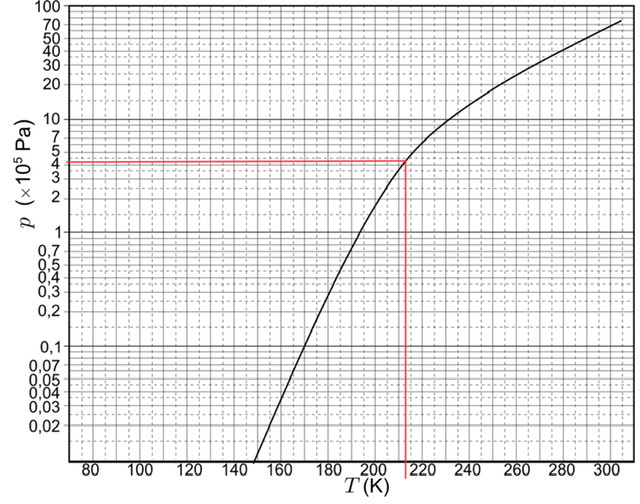
\includegraphics[width=15cm]{thermo78.jpeg}
\end{center}
\end{solution}